\section{First occurrence, rigidity, and defect constraints}
\label{sec:first-rigidity}

Exact solvability does not explain why period eight is the first strict
crossing of the reference edge.  That question depends on the arrangement of
local cancellations.  Squaring the operator turns those cancellations into a
defect geometry that can be measured by short closed walks.

\subsection{Local squares and moments}

Put $Q_i=\tau_i\tau_{i+1}$.  Direct multiplication of
\eqref{eq:hamilton-operator} gives
\begin{align}
(A_\tau^2x)_i={}&4x_i+x_{i-2}+x_{i+2}
 +\tau_{i-4}\tau_{i-2}x_{i-4}+\tau_i\tau_{i+2}x_{i+4}\notag\\
&+\tau_{i-3}(1+Q_{i-3})x_{i-3}
 +\tau_{i-2}(1+Q_{i-2})x_{i-1}\notag\\
&+\tau_{i-1}(1+Q_{i-1})x_{i+1}
 +\tau_i(1+Q_i)x_{i+3}.
\label{eq:local-square-row}
\end{align}
Thus $Q_i=-1$ cancels the corresponding odd-displacement coupling, whereas
$Q_i=1$ activates a term of absolute value two.  A positive $Q$-site will be
called a defect.

For a $p$-periodic word, define
\begin{equation}
 M_k(\tau)=\frac1{2\pi}\int_0^{2\pi}
 \tr\!\left(H_\tau^{(p)}(e^{\mathrm i\theta})^{2k}\right)d\theta.
 \label{eq:phase-averaged-moments}
\end{equation}
Let $d$ be the number of defects and set
\begin{equation}
 a=\#\{i:Q_i=Q_{i+1}=1\},\qquad
 b=\#\{i:Q_i=Q_{i+2}=1\}.
 \label{eq:defect-statistics}
\end{equation}
The diagonal and squared row norm in \eqref{eq:local-square-row} give $M_1$
and $M_2$.  At length six, the closed step words have four translation classes
of $Q$-support:
\begin{equation}
 M_3=\sum_{i=0}^{p-1}
 \left(238+156Q_i+24Q_iQ_{i+1}+12Q_iQ_{i+2}\right).
 \label{eq:m3-q-expansion}
\end{equation}
The four normalized supports and their closed-step multiplicities are
\[
\begin{array}{c|cccc}
\text{support}&\varnothing&\{0\}&\{0,1\}&\{0,2\}\\ \hline
\text{multiplicity}&238&156&24&12.
\end{array}
\]
Conversion from the sign monomials to defect statistics uses
\[
 \sum_iQ_i=2d-p,\quad
 \sum_iQ_iQ_{i+1}=4a-4d+p,\quad
 \sum_iQ_iQ_{i+2}=4b-4d+p,
\]
we obtain the human-checkable formulas
\begin{equation}
 M_1=4p,\qquad M_2=20p+16d,\qquad
 M_3=118p+168d+96a+48b.
 \label{eq:first-three-moments}
\end{equation}
Here $(1+Q_i)^2=2(1+Q_i)$ explains the $16d$ in $M_2$.
The next moment sees individual defects through $d$ and their interactions at
distances one and two through $a$ and $b$.

If $R_p(\tau)\leq8$, every squared fiber eigenvalue $y$ lies in $[0,8]$.
Hence $M_{k+1}\leq8M_k$, and $k=1,2$ gives
\begin{equation}
 d\leq\frac{3p}{4},\qquad
 40d+96a+48b\leq42p.
 \label{eq:moment-excess-inequalities}
\end{equation}
The first bound controls defect density; the second also penalizes short-range
clustering.

\subsection{Periods below eight}

Legality gives $\prod_iQ_i=1$, or $d\equiv p\pmod2$.  For $d>0$, record a
word by the positive cyclic gaps between consecutive defects.  The gaps sum
to $p$ and are considered up to cyclic permutation and reversal.  Combining
these gap compositions with \eqref{eq:moment-excess-inequalities} gives the
complete table
\begin{equation}
\begin{array}{c|c|l}
p&(d,a,b)&\text{surviving dihedral representatives}\\ \hline
1&-&\text{none}\\
2&(0,0,0)&--\\
3&(1,0,0)&--+\\
4&(0,0,0)&----\\
5&(1,0,0)&----+\\
6&(0,0,0)&------\\
 &(2,1,0),(2,0,1),(2,0,0)&----++,\;---+-+,\;--+--+\\
7&(1,0,0)&------+\\
 &(3,1,1),(3,1,0),(3,0,2)&---+-++,\;--+--++,\;--+-+-+
\end{array}
\label{eq:short-survivors}
\end{equation}
Indeed, parity and the density bound leave only the displayed values of $d$.
Listing the cyclic compositions of $p$ for those values and substituting
$a,b$ in the second bound gives exactly the middle column; each triple has the
stated dihedral representative.  This proves completeness before any matrix
certificate is used.

The all-negative words have even period; their lifts alternate and have edge
$8$.  For the other rows choose the lift with $\tau_0=1$ and put
$C_\tau(z)=8I-H_\tau^{(p)}(z)^2$.  A negative Rayleigh value for $C_\tau(z)$
excludes edge at most $8$.

\begin{lemma}
\label{lem:short-certificates}
For the $p=3$ representative, at $z=e^{\pi\mathrm i/3}$,
$\det C_\tau(z)=-1$.  For every other nonbalanced representative,
Table~\ref{tab:certificates} gives $v^*C_\tau(z)v<0$.
\end{lemma}

\begin{table}[t]
\centering
\caption{Exact Rayleigh certificates after the moment and dihedral
reductions.  The last column is $v^*(8I-H^2)v$.}
\label{tab:certificates}
\scriptsize
\begin{tabularx}{\textwidth}{@{}c l c >{\raggedright\arraybackslash}X r@{}}
\toprule
$p$&$Q$&$z$&$v$&value\\ \midrule
5&$----+$&$1$&$(1,1,1,0,1)$&$-4$\\
6&$----++$&$1$&$(1,1,1,0,1,1)$&$-12$\\
6&$---+-+$&$-1$&$(0,0,2,-1,2,-2)$&$-4$\\
6&$--+--+$&$\mathrm i$&$(3+\mathrm i,3,3+2\mathrm i,1+3\mathrm i,
2+2\mathrm i,4\mathrm i)$&$-4$\\
7&$------+$&$1$&$(1,1,1,0,1,0,1)$&$-2$\\
7&$---+-++$&$1$&$(1,1,1,0,0,1,1)$&$-4$\\
7&$--+--++$&$1$&$(1,1,1,1,1,1,1)$&$-8$\\
7&$--+-+-+$&$-1$&$(1,1,1,1,1,1,-1)$&$-8$\\ \bottomrule
\end{tabularx}
\end{table}

\begin{proof}
Each table row is one direct multiplication in order at most seven.  Its
negative value makes $C_\tau(z)$ indefinite.  In the $p=3$ case,
$C_\tau(e^{\pi\mathrm i/3})$ is Hermitian and has negative determinant, so it
also has a negative eigenvalue.
\end{proof}

\begin{theorem}
\label{thm:minimal-period}
No legal word of primitive period below eight has squared Bloch edge below
$8$.  The word $\tau_*$ has primitive period eight and edge $\etaedge<8$.
\end{theorem}

\begin{proof}
The displayed-period assertion follows from
\eqref{eq:short-survivors} and Lemma~\ref{lem:short-certificates}.
Zone folding \eqref{eq:zone-folding} shows that cell repetition does not
change the edge.  Finally $\tau_{i+4}=-\tau_i$ excludes period four, and its
first four signs exclude periods one and two.
\end{proof}

The period-two reference is already chiral, but remains on the boundary
$R_2=8$; all primitive periods below eight remain on or above that boundary.
Period eight is therefore the first point at which the half-cell mechanism is
spectrally effective rather than merely present.  This proves
Theorem~\ref{thm:main-minimal} and leaves the internal structure of the first
feasible period to be determined.

\FloatBarrier
\subsection{Rigidity at period eight}

For $p=8$, legality and \eqref{eq:moment-excess-inequalities} leave the
all-negative word and four two-defect words up to dihedral symmetry.  Their
defect separations are $1,2,3,4$; separation $4$ is the antipodal word $Q_*$.
Figure~\ref{fig:defect-orbits} shows the four orbits through their defect
positions; the signs between the marked positions are recovered from the
cyclic gap word.

\begin{figure}[t]
 \centering
 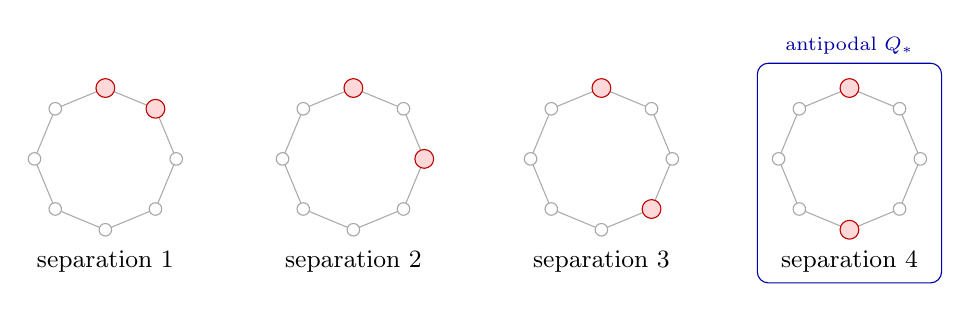
\begin{tikzpicture}[scale=.9,
 dot/.style={circle,draw=gray!70,fill=white,inner sep=1.6pt},
 defect/.style={circle,draw=red!75!black,fill=red!15,inner sep=2.4pt}]
\foreach \sep/\x/\lab in {1/0/$1$,2/3.5/$2$,3/7/$3$,4/10.5/$4$}{
  \begin{scope}[xshift=\x cm]
    \draw[gray!65] (0:1)--(45:1)--(90:1)--(135:1)--(180:1)--(225:1)--(270:1)--(315:1)--cycle;
    \foreach \j in {0,...,7}{\node[dot] (n\sep-\j) at ({90-45*\j}:1) {};}
    \node[defect] at (n\sep-0) {};
    \node[defect] at (n\sep-\sep) {};
    \node[font=\small] at (0,-1.45) {separation \lab};
    \ifnum\sep=4
      \draw[blue!65!black,rounded corners] (-1.3,-1.75) rectangle (1.3,1.35);
      \node[blue!65!black,font=\scriptsize] at (0,1.6) {antipodal $Q_*$};
    \fi
  \end{scope}
}
\end{tikzpicture}

 \caption{The four period-eight two-defect geometries modulo the dihedral
 action.  The first three separations have edge above $8$; the antipodal orbit
 $Q_*$ is the unique sub-eight orbit.}
 \label{fig:defect-orbits}
\end{figure}

The first three configurations are distinguished by one integer closed-walk
recurrence.  If $f_\ell^{(r)}(j)$ is the signed walk sum of length $\ell$ from
$r$ to $j$, with $f_0^{(r)}(j)=\delta_{rj}$, then
\begin{equation}
 f_{\ell+1}^{(r)}(j)=f_\ell^{(r)}(j-1)+f_\ell^{(r)}(j+1)
 +\tau_{j-2}f_\ell^{(r)}(j-2)+\tau_jf_\ell^{(r)}(j+2).
 \label{eq:walk-recurrence}
\end{equation}
Set $E_k=M_{k+1}-8M_k$.  Edge at most $8$ would imply $E_k\leq0$.

\begin{lemma}
\label{lem:period8-recurrence}
For defect separations $1,2,3$, recurrence \eqref{eq:walk-recurrence} gives,
respectively,
\begin{equation}
 (k,E_k)=(4,5504),\qquad(6,64336),\qquad(9,2872096).
 \label{eq:period8-excesses}
\end{equation}
Consequently each nonantipodal two-defect word has edge above $8$.
\end{lemma}

\begin{proof}
The recurrence uses only integer addition and multiplication by the displayed
signs.  Summing $f_{2k}^{(r)}(r)$ over one period gives $M_k$; iteration to the
listed $k$ gives the three positive excesses, contradicting $E_k\leq0$.
\end{proof}

\begin{theorem}
\label{thm:period8-trichotomy}
Among legal period-eight $Q$-words, $Q_*$ is the unique dihedral orbit with
squared Bloch edge below $8$.  Its two $\tau$-lifts differ by a global sign and
have the same squared edge.  The all-negative $Q$-word has edge $8$, and every
other orbit has edge above $8$.
\end{theorem}

\begin{proof}
The all-negative lift is the period-two reference.  The antipodal orbit has
edge $\etaedge<8$ by Section~\ref{sec:period8}, and
Lemma~\ref{lem:period8-recurrence} excludes the other three two-defect orbits.
Proposition~\ref{prop:invariances} justifies the dihedral quotient and
identifies the two lifts spectrally.
\end{proof}

The survivor has two defects at the largest possible cyclic separation.
This geometry matches the moments: $M_2$ penalizes the number of activated
sites, while $M_3$ adds penalties at separations one and two.  At period eight
these restrictions, followed by the exact recurrence, become a complete
trichotomy.  For arbitrary periods they remain necessary constraints.

\subsection{A general consequence}

The moment identities did not use $p\leq8$.  For any legal periodic word,
$R_p(\tau)\leq8$ implies
\begin{equation}
 d\leq\frac{3p}{4},\qquad 40d+96a+48b\leq42p.
 \label{eq:general-defect-bounds}
\end{equation}
Thus low edge requires controlled defect density and controlled short-range
clustering.  These conditions do not characterize longer-period phases or
determine the global minimum in \eqref{eq:fixed-minimum}; they expose the
general local geometry whose first complete realization is the rigid
period-eight orbit.
